
\documentclass[../main/SI3_manual]{subfiles}

\begin{document}

% ================================================================
% Chapter 2 � Domain
% ================================================================

\chapter{Time, space and thickness space domain}
\label{chap:DOM}
\chaptertoc

\newpage
$\ $\newline    % force a new line

Having defined the model equations in previous Chapter, we need now to choose the numerical discretization.  In the present chapter, we provide a general description of the SI$^3$ discretization strategy, in terms of time, space and thickness, which is considered as an extra independent variable. 

Sea ice state variables are typically expressed as:
\begin{equation}
X(ji,jj,\textcolor{gray}{jk},jl).
\end{equation}
$ji$ and $jj$ are x-y spatial indices, as in the ocean. $jk=1, ..., nlay\_i$ corresponds to the vertical coordinate system in sea ice (ice layers), and only applies to vertically-resolved quantities (ice enthalpy and salinity). $jl=1, ..., jpl$ corresponds to the ice categories, discretizing thickness space.

\section{Time domain}

%--------------------------------------------------------------------------------------------------------------------
%
% FIG x : Time Stepping
%
\begin{figure}[ht]
\begin{center}
\vspace{0cm}
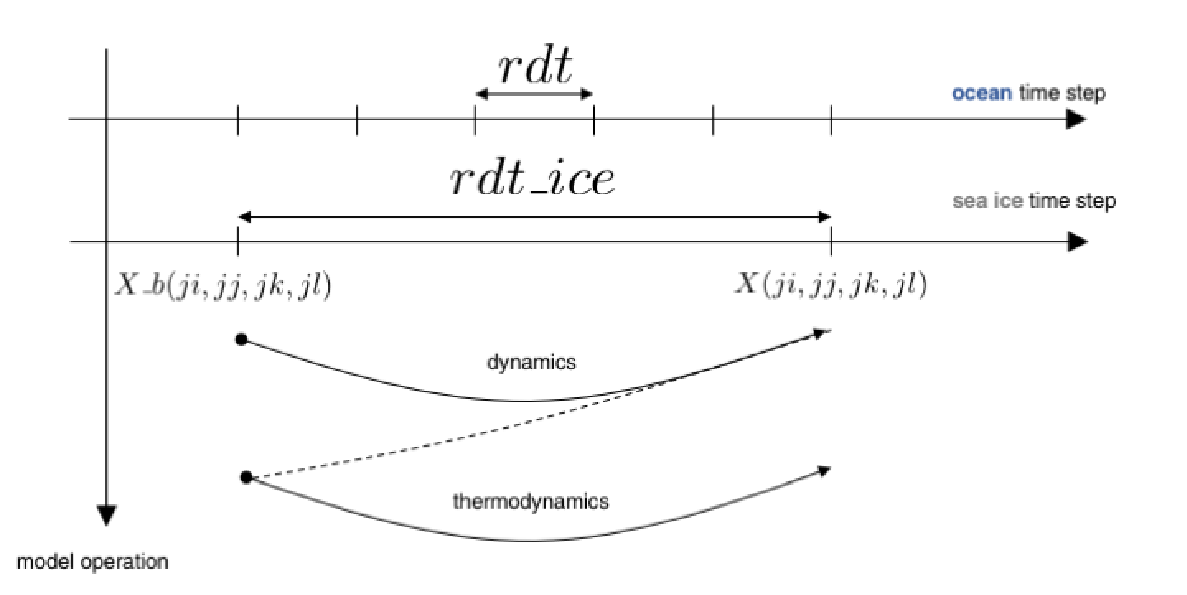
\includegraphics[height=6cm,angle=-00]{time_stepping}
\caption{Schematic representation of time stepping in SI$^3$, assuming $nn\_fsbc=5$.}
\label{ice_scheme}
\end{center}
\end{figure}
%
%--------------------------------------------------------------------------------------------------------------------

The sea ice time stepping is synchronized with that of the ocean. Because of the potentially large numerical cost of sea ice physics, in particular rheology, SI$^3$ can be called every nn\_fsbc time steps (namsbc in \textit{namelist\_ref}). The sea ice time step is therefore $rdt\_ice = rdt * nn\_fsbc$. In terms of quality, the best value for \textit{nn\_fsbc} is 1, providing full consistency between sea ice and oceanic fields. Larger values (typically 2 to 5) can be used but numerical instabilities can appear because of the progressive decoupling between the state of sea ice and that of the ocean, hence changing $nn\_fsbc$ must be done carefully.

Ice dynamics (rheology, advection, ridging/rafting) and thermodynamics are called successively. To avoid pathological situations, thermodynamics were chosen to be applied on fields that have been updated by dynamics, in a somehow semi-implicit procedure.

There are a few iterative / subcycling procedures throughout the code, notably for rheology, advection, ridging/ rafting and the diffusion of heat. In some cases, the arrays at the beginning of the sea ice time step are required. Those are referred to as $X\_b$.

\section{Spatial domain}

%--------------------------------------------------------------------------------------------------------------------
%
% FIGx : Vertical grid
%
%
\begin{figure}[!ht]
\begin{center}
\vspace{0cm}
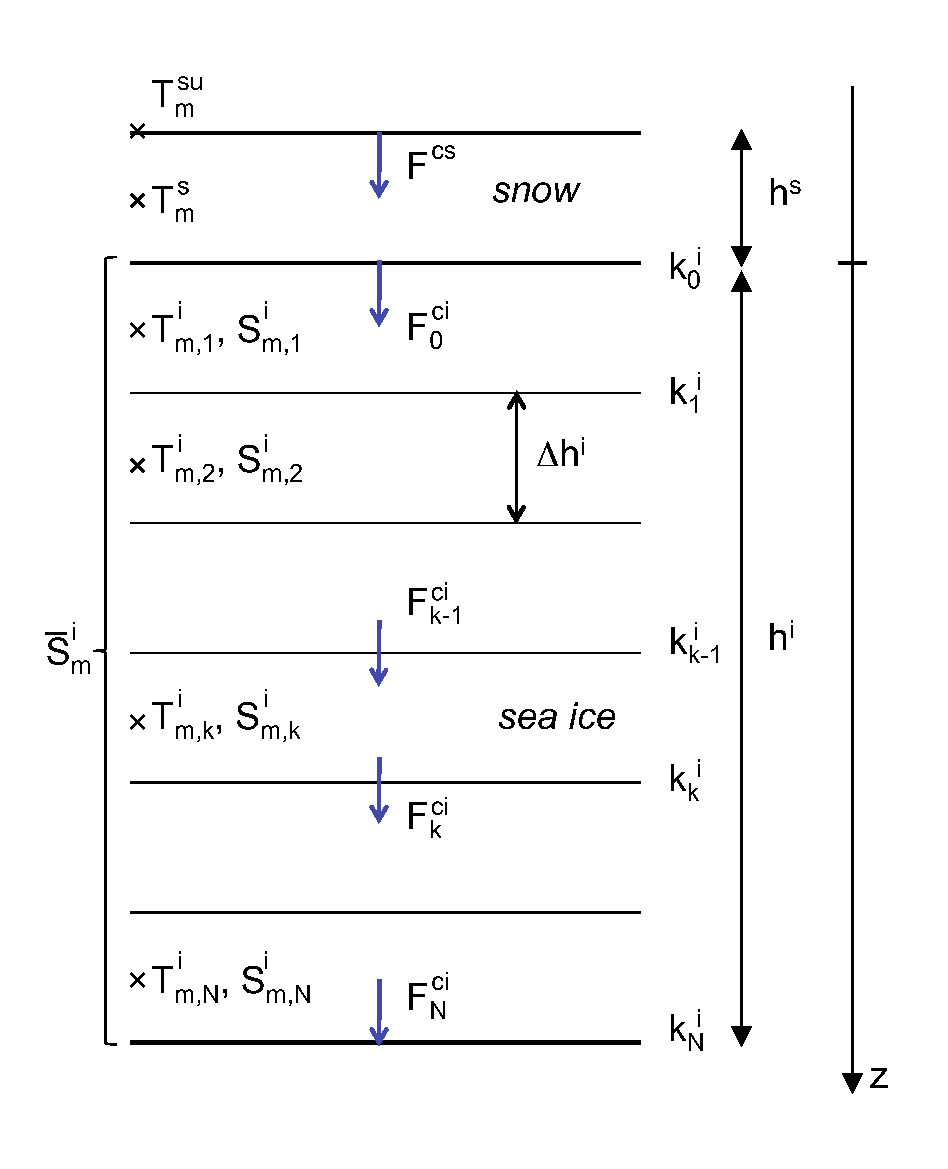
\includegraphics[height=10cm,angle=-00]{thermogrid.eps}
\caption{\footnotesize{Vertical grid of the model, used to resolve vertical temperature and salinity profiles}}\label{fig_dom_icelayers}
\end{center}
\end{figure}
%
%--------------------------------------------------------------------------------------------------------------------

The horizontal indices $ji$ and $jj$ are handled as for the ocean in NEMO, assuming C-grid discretization and in most cases a finite difference expression for scale factors.

The vertical index $jk=1, ..., nlay\_i$ is used for enthalpy (temperature) and salinity. In each ice category, the temperature and salinity profiles are vertically resolved over $nlay\_i$ equally-spaced layers. The number of snow layers can currently only be set to $nlay\_s=1$ (Fig. \ref{fig_dom_icelayers}).

To increase numerical efficiency of the code, the two horizontal dimensions of an array $X(ji,jj,jk,jl)$ are collapsed into one (array $X\_1d(ji,jk,jl)$) for thermodynamic computations, and re-expanded afterwards.

\nlst{nampar}

\section{Thickness space domain}

\nlst{namitd}

Thickness space is discretized using $jl=1, ..., jpl$ thickness categories, with prescribed boundaries $hi\_max(jl-1),hi\_max(jl)$. Following \cite{lipscomb_2001}, ice thickness can freely evolve between these boundaries. The number of ice categories $jpl$ can be adjusted from the namelist ($nampar$).

There are two means to specify the position of the thickness boundaries of ice categories. The first option (ln\_cat\_hfn) is to use a fitting function that places the category boundaries between 0 and 3$\overline h$, with $\overline h$ the expected mean ice thickness over the domain (namelist parameter rn\_himean), and with a greater resolution for thin ice (Fig. \ref{fig_dom_icecats}). More specifically, the upper limits for ice in category $jl=1, ..., jpl-1$ are:
\begin{eqnarray} 
hi\_max(jl) = \biggr ( \frac{jl \cdot (3\overline h + 1 )^{\alpha}}{ (jpl-jl)(3 \overline h + 1)^{\alpha} + jl }\biggr )^{\alpha^{-1}} - 1,
\end{eqnarray}
with $hi\_max(0)$=0 m and $\alpha = 0.05$. The last category has no upper boundary, so that it can contain arbitrarily thick ice.

%--------------------------------------------------------------------------------------------------------------------
%
% FIGx : Ice categories
%
%
\begin{figure}[!ht]
\begin{center}
\vspace{0cm}
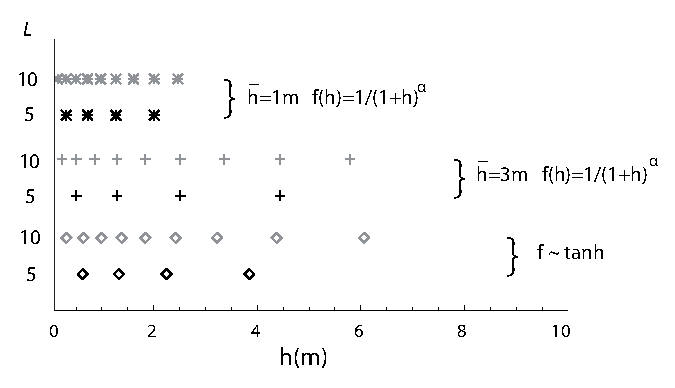
\includegraphics[height=6cm,angle=-00]{ice_cats.eps}
\caption{\footnotesize{Boundaries of the model ice thickness categories (m) for varying number of categories and prescribed mean thickness ($\overline h$). The formerly used $tanh$ formulation is also depicted.}}\label{fig_dom_icecats}
\end{center}
\end{figure}
%
%--------------------------------------------------------------------------------------------------------------------

The other option (ln\_cat\_usr) is to specify category boundaries by hand using rn\_catbnd. The first category must always be thickner than rn\_himin (0.1 m by default).

The choice of ice categories is important, because it constraints the ability of the model to resolve the ice thickness distribution. The latest study \citep{massonnet_2018} recommends to use at least 5 categories, which should include one thick ice with lower bounds at $\sim$4 m and $\sim$2 m for the Arctic and Antarctic, respectively, for allowing the storage of deformed ice.

With a fixed number of cores, the cost of the model linearly increases with the number of ice categories. Using $jpl=1$ single ice category is also much cheaper than with 5 categories, but seriously deteriorates the ability of the model to grow and melt ice. Indeed, thin ice thicknes faster than thick ice, and shrinks more rapidly as well. When nn\_virtual\_itd=1 ($jpl$ = 1 only), two parameterizations are activated to compensate for these shortcomings. Heat conduction and areal decay of melting ice are adjusted to closely approach the 5 categories case.

\end{document}